\section{Nutzerhandbuch Navigations"=App}
Die Projektgruppe RIO bietet eine Anwendung für Handynutzer, mit deren Hilfe Sie in Oldenburg anhand Umwelt Parametern navigieren können.\\
Die folgenden Schritte zeigen Ihnen, wie Sie die App einrichten und benutzen können.
 
\subsection{Anwendung starten}

\begin{itemize}
	\item Laden Sie die RIO Navigation Anwendung herunter und installieren Sie diese.
  \item Öffnen Sie auf Ihrem Handy die RIO Navigation Anwendung.
  \item Tippen Sie oben links auf die Menüschaltfläche, um die Routeninformationen zu öffnen.
\end{itemize}
Wie gezeigt in \Fig{app:starten}.
\begin{figure}[h!]
\centerline{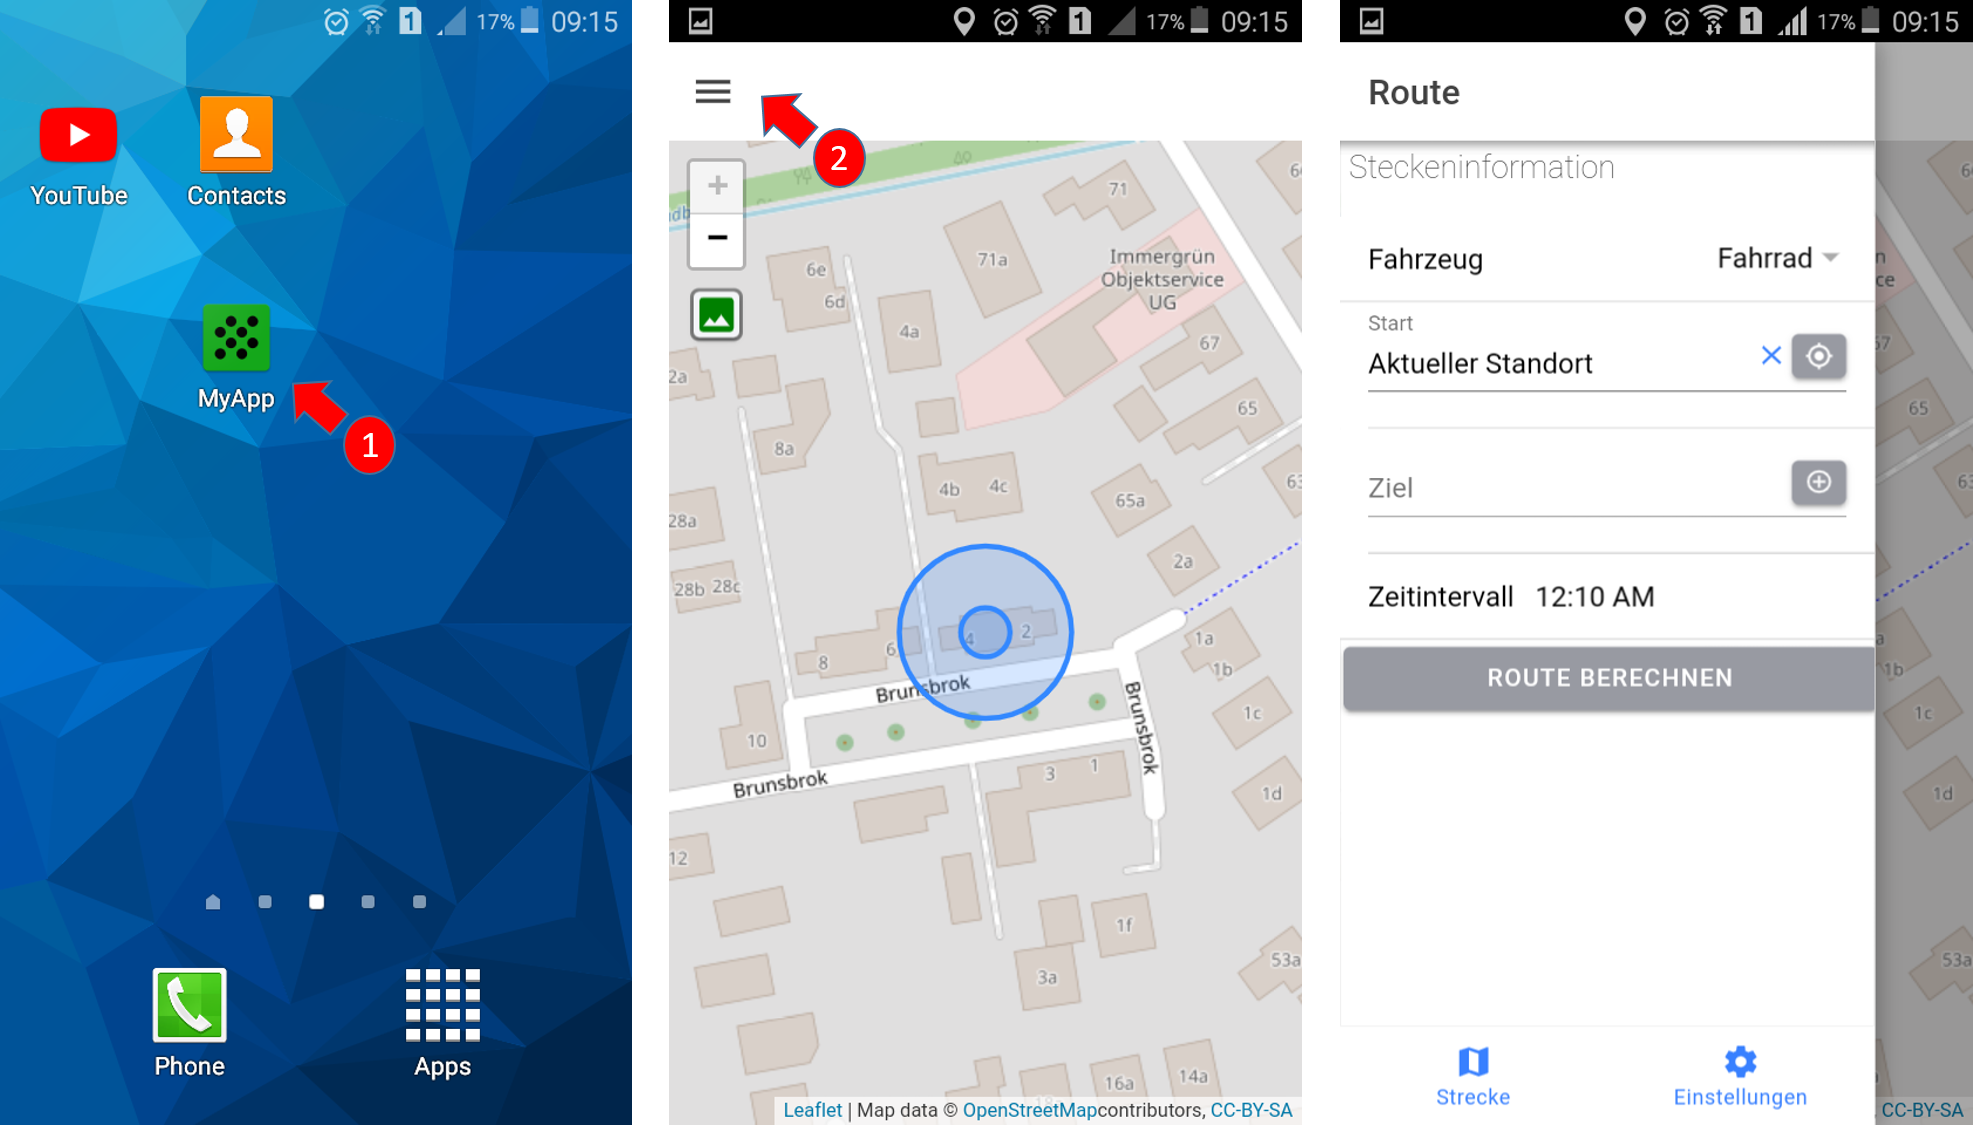
\includegraphics[height=8 cm]{./ressourcen/nutzerhandbuch/start_up.png}}
\caption{RIO Navigation Anwendung starten.}
\label{fig:app:starten}
\end{figure}

\newpage
\subsection{Route berechnen und Routen anzeigen}
\paragraph{Startpunkt:}
Suchen Sie nach Ihrem Start oder tippen Sie auf der Karte auf den gewünschten Startpunkt.\\
Wie gezeigt in \Fig{app:Startpunkt}.
\begin{figure}[h!]
\centerline{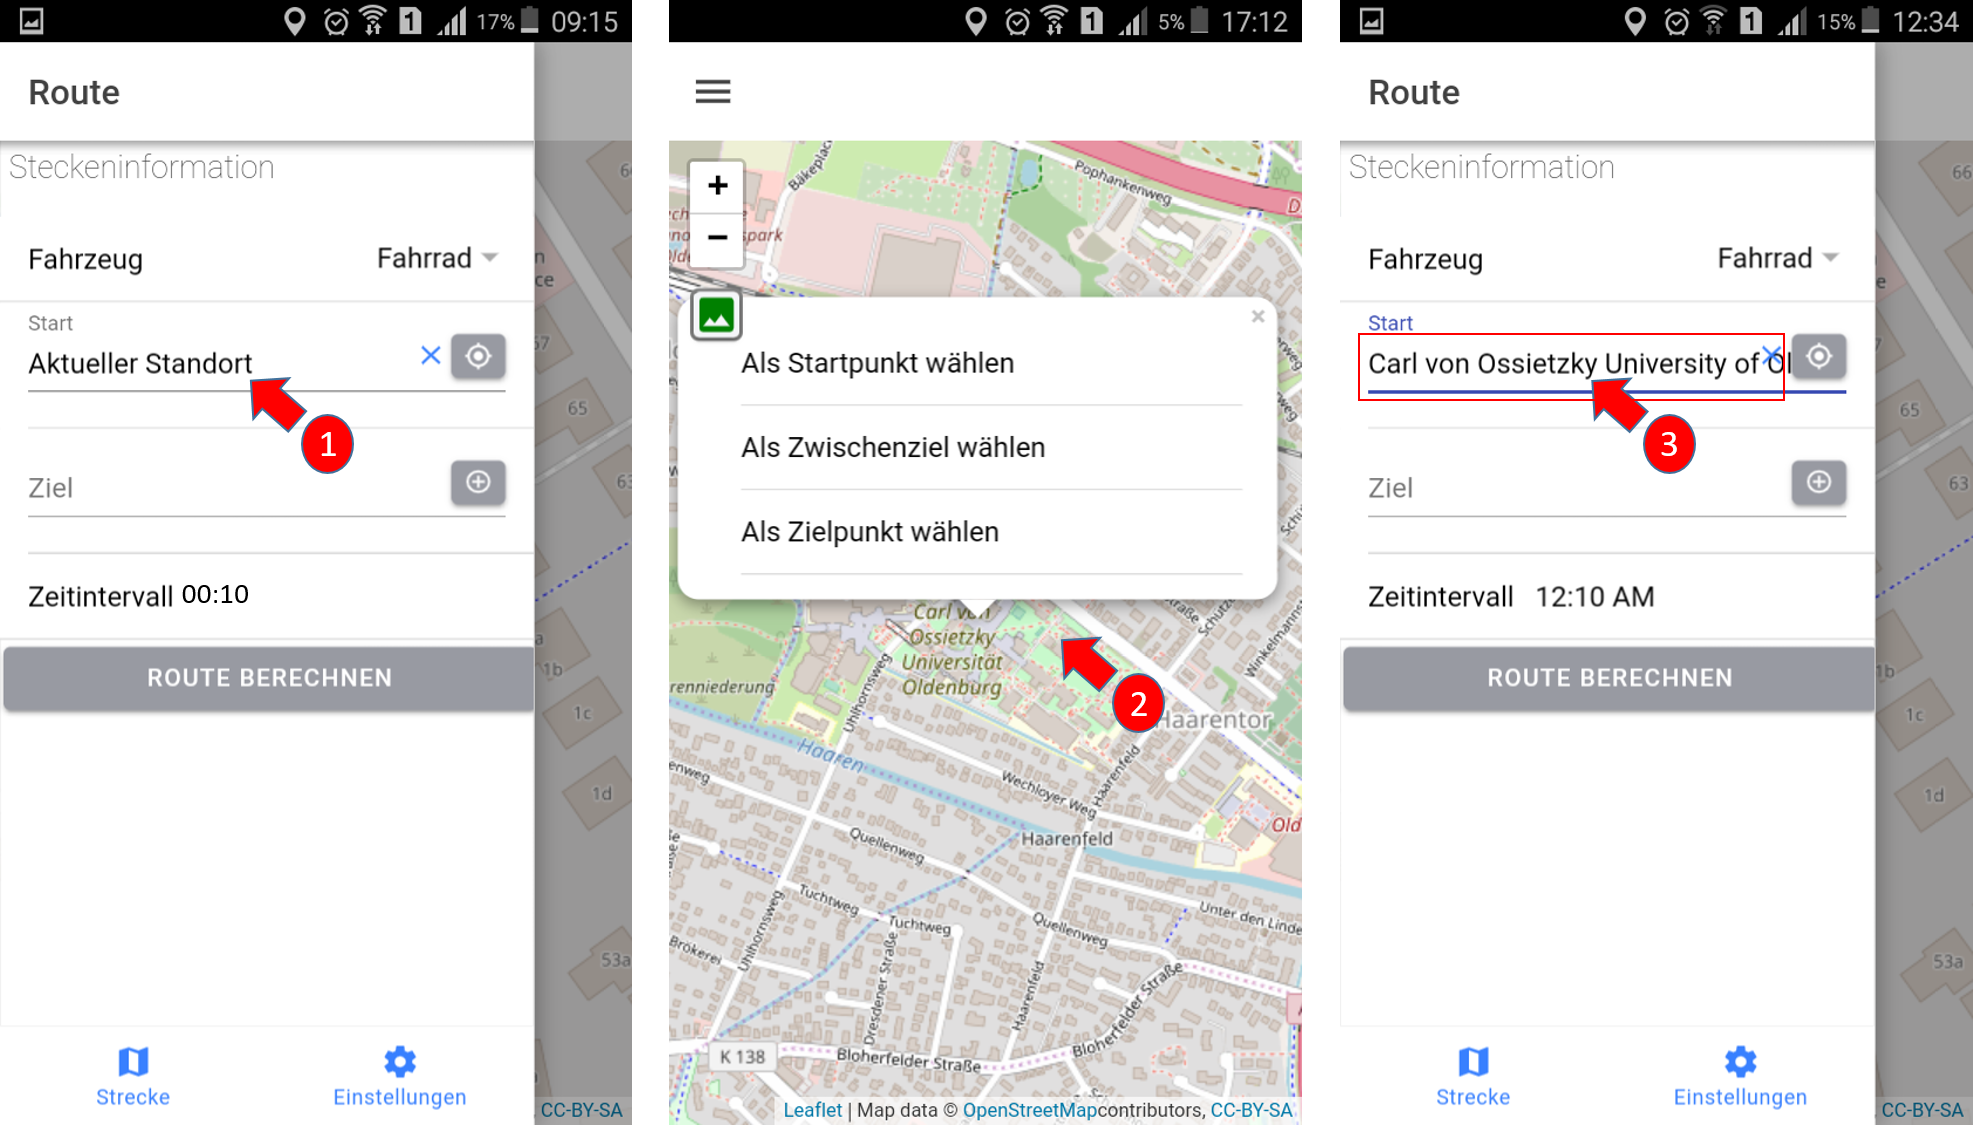
\includegraphics[height=8 cm]{./ressourcen/nutzerhandbuch/start.png}}
\caption{Startpunkt wählen}
\label{fig:app:Startpunkt}
\end{figure} 

\newpage

\paragraph{Zwischenziele:}
\begin{itemize}
  \item Um ein Zwischenziel hinzuzufügen, klicken Sie auf das Plus-Symbol rechts neben dem Zieleingabefeld.
  \item Suchen Sie nach Ihrem Zwischenziel oder tippen Sie auf der Karte auf das gewünschte Zwischenziel.
\end{itemize}
Wie gezeigt in \Fig{app:Zwischenziel}.
\begin{figure}[h!]
\centerline{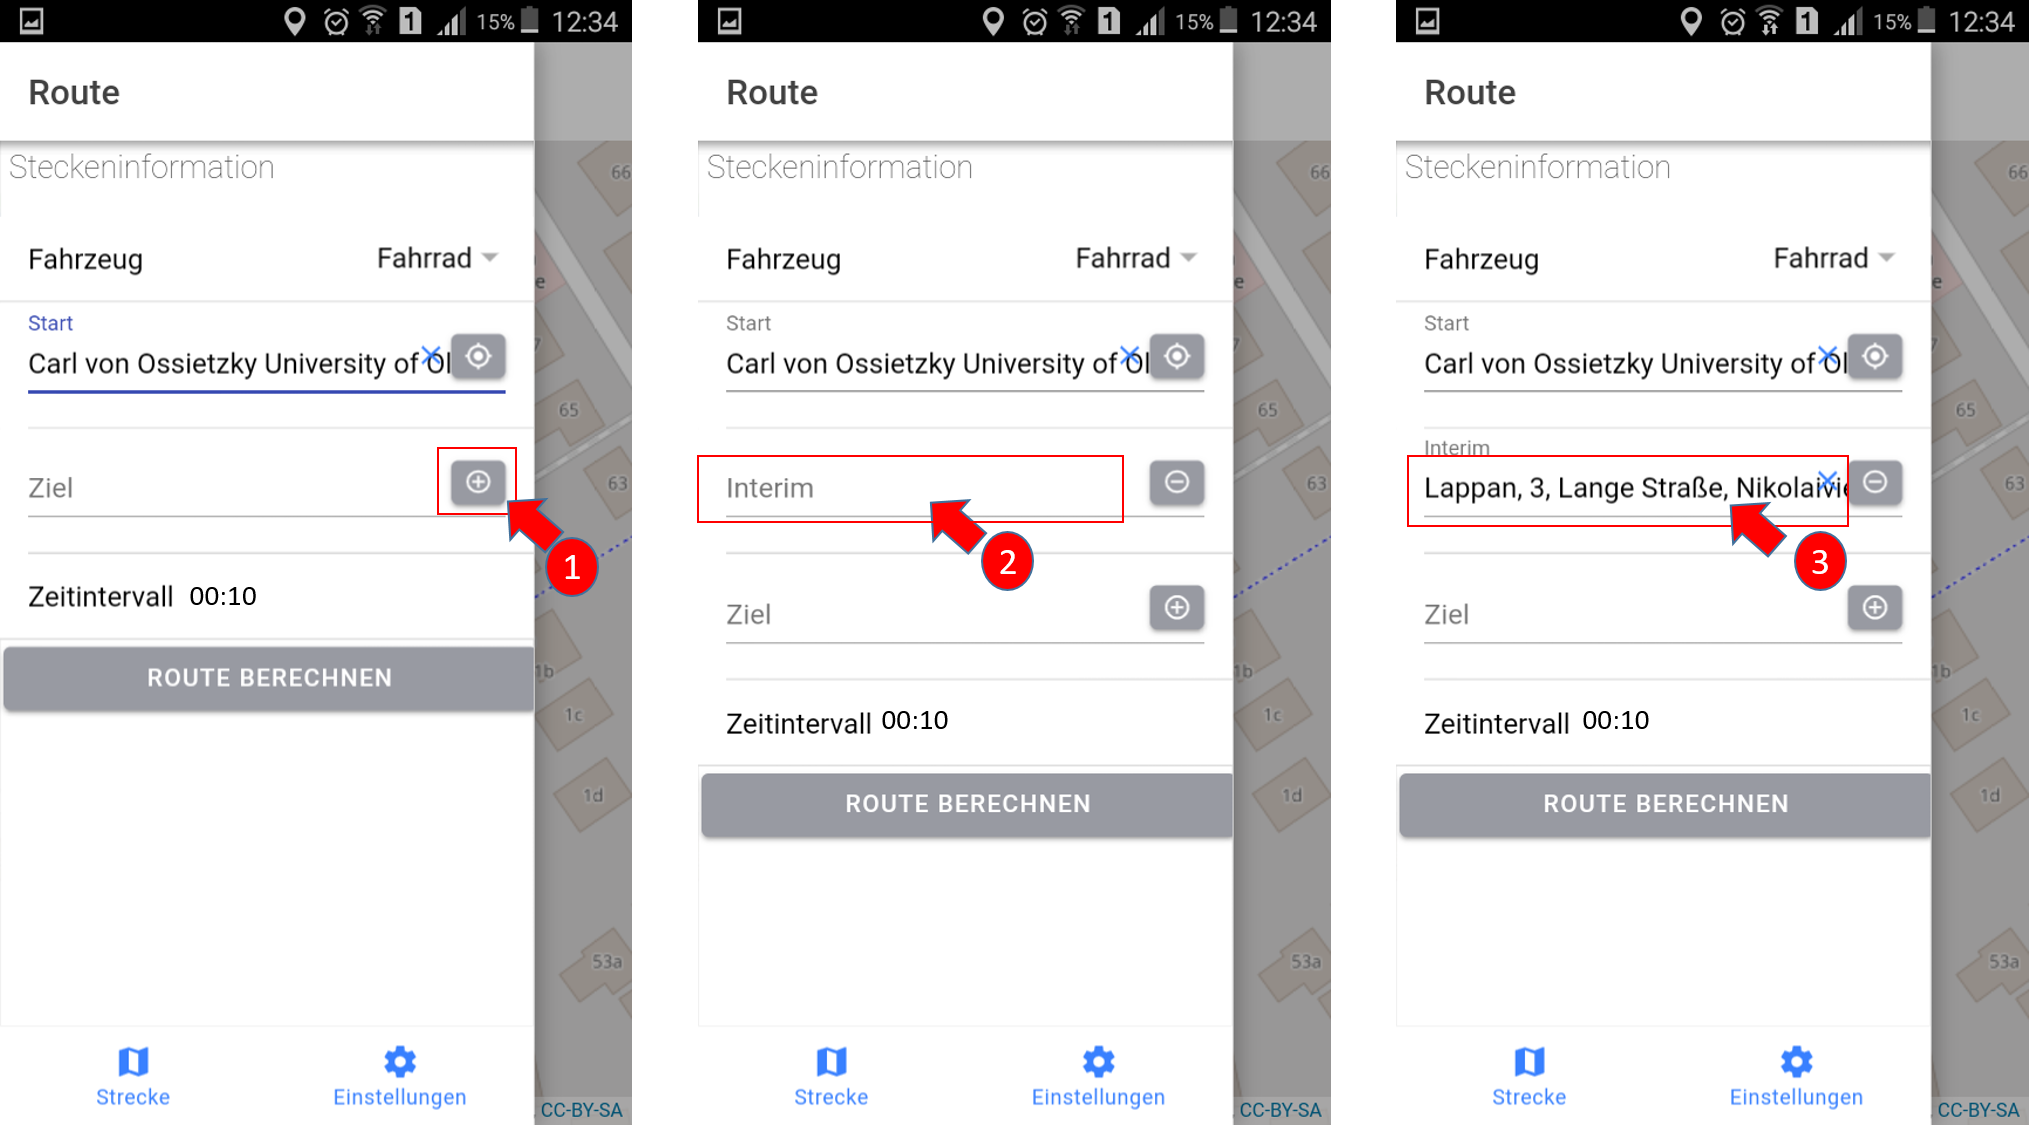
\includegraphics[height=8 cm]{./ressourcen/nutzerhandbuch/intrim.png}}
\caption{Zwischenziel hinzufügen}
\label{fig:app:Zwischenziel}
\end{figure} 

\newpage

\paragraph{Zielpunkt:}
Suchen Sie nach Ihrem Ziel oder tippen Sie auf der Karte auf das gewünschte Ziel.\\
Wie gezeigt in \Fig{app:Zielpunkt}.
\begin{figure}[h!]
\centerline{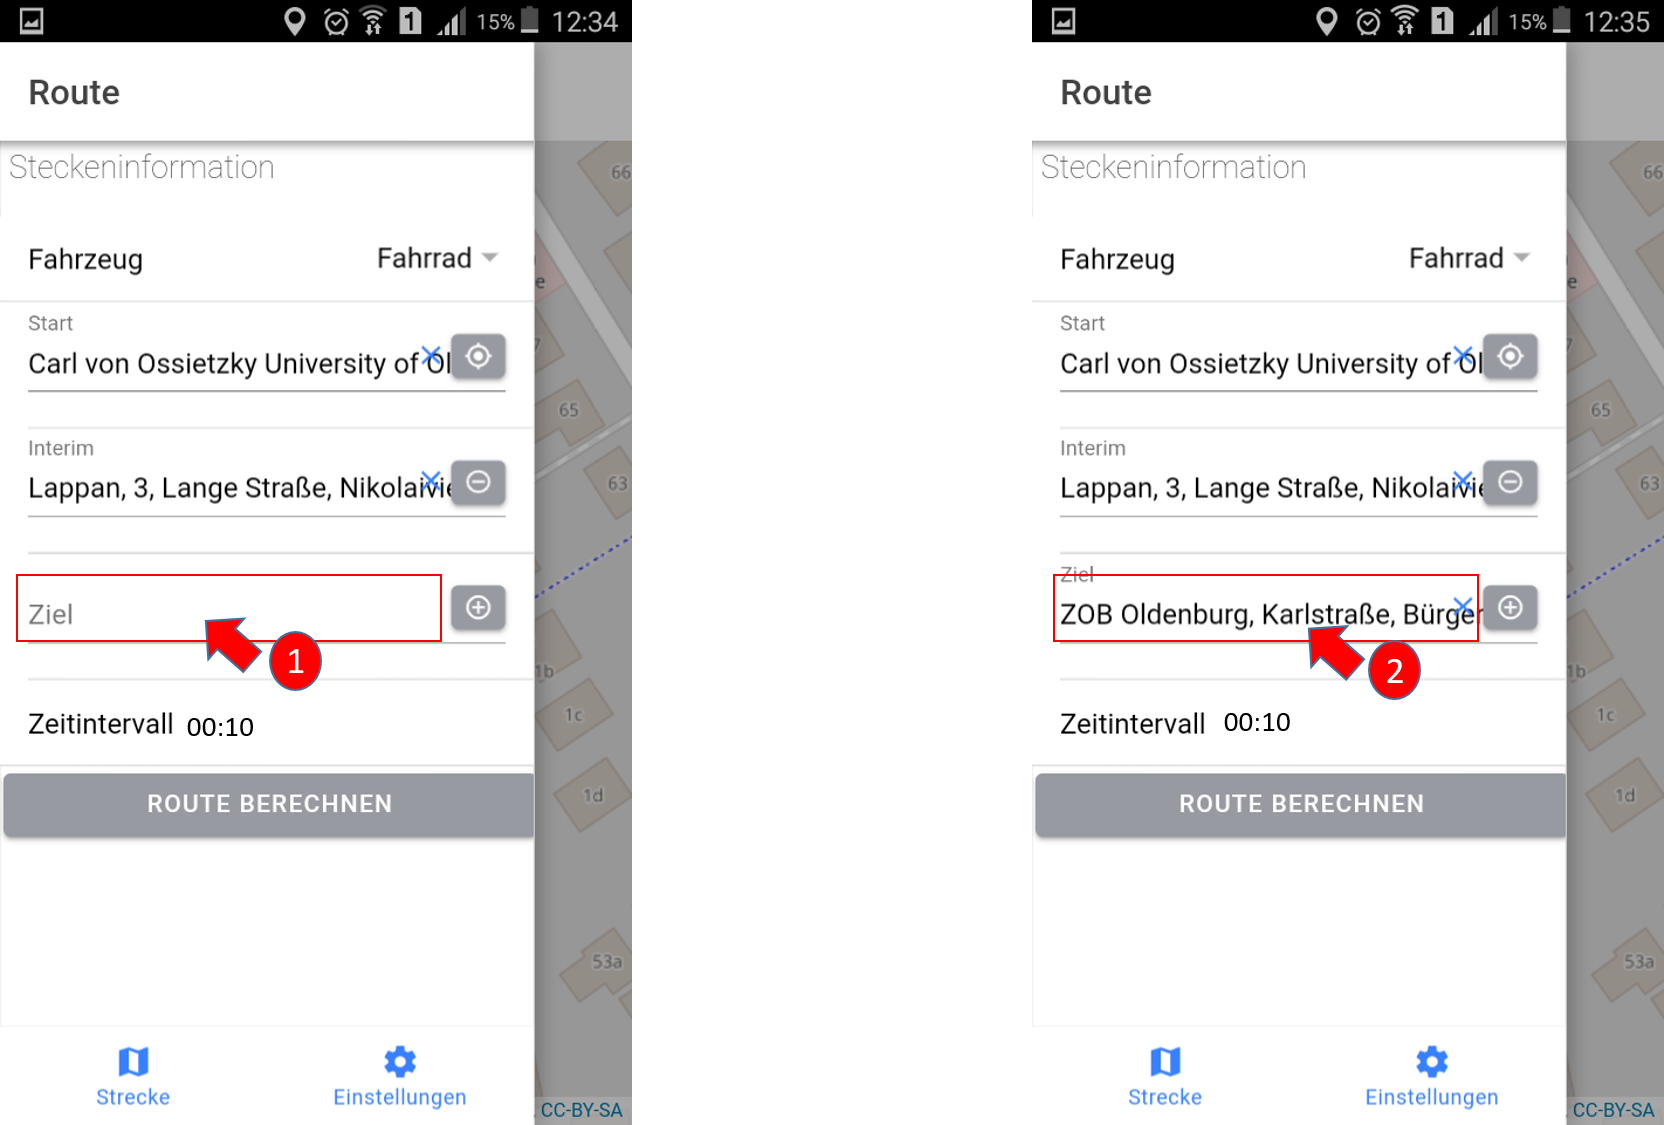
\includegraphics[height=8 cm]{./ressourcen/nutzerhandbuch/ziel.png}}
\caption{Zielpunkt}
\label{fig:app:Zielpunkt}
\end{figure}
 
\newpage
\paragraph{Routeneinstellungen:}
\begin{itemize}
  \item Tippen Sie auf die Schaltfläche Einstellungen, um die Routing-Einstellungen zu öffnen.\\
  Wie gezeigt in \Fig{app:Routeneinstellungen}.
  \item Wählen Sie Ihre Einstellungen für Umgebungsparameter. Diese Parameter haben Einfluss auf die Routenberechnung.
  	\begin{itemize}
  		\item Wählen Sie die maximalen PM10-Feinstaub- und Relevanzwerte.
  		\item Wählen Sie die maximalen PM25-Feinstaub- und Relevanzwerte.
  		\item Wählen Sie die minimalen und maximalen Temperaturwerte und die Relevanz der Temperatur.
	\end{itemize}
  \item Tippen Sie auf die Schaltfläche Strecke, um zur  Streckeninformation zurückzukehren
\end{itemize}

\begin{figure}[h!]
\centerline{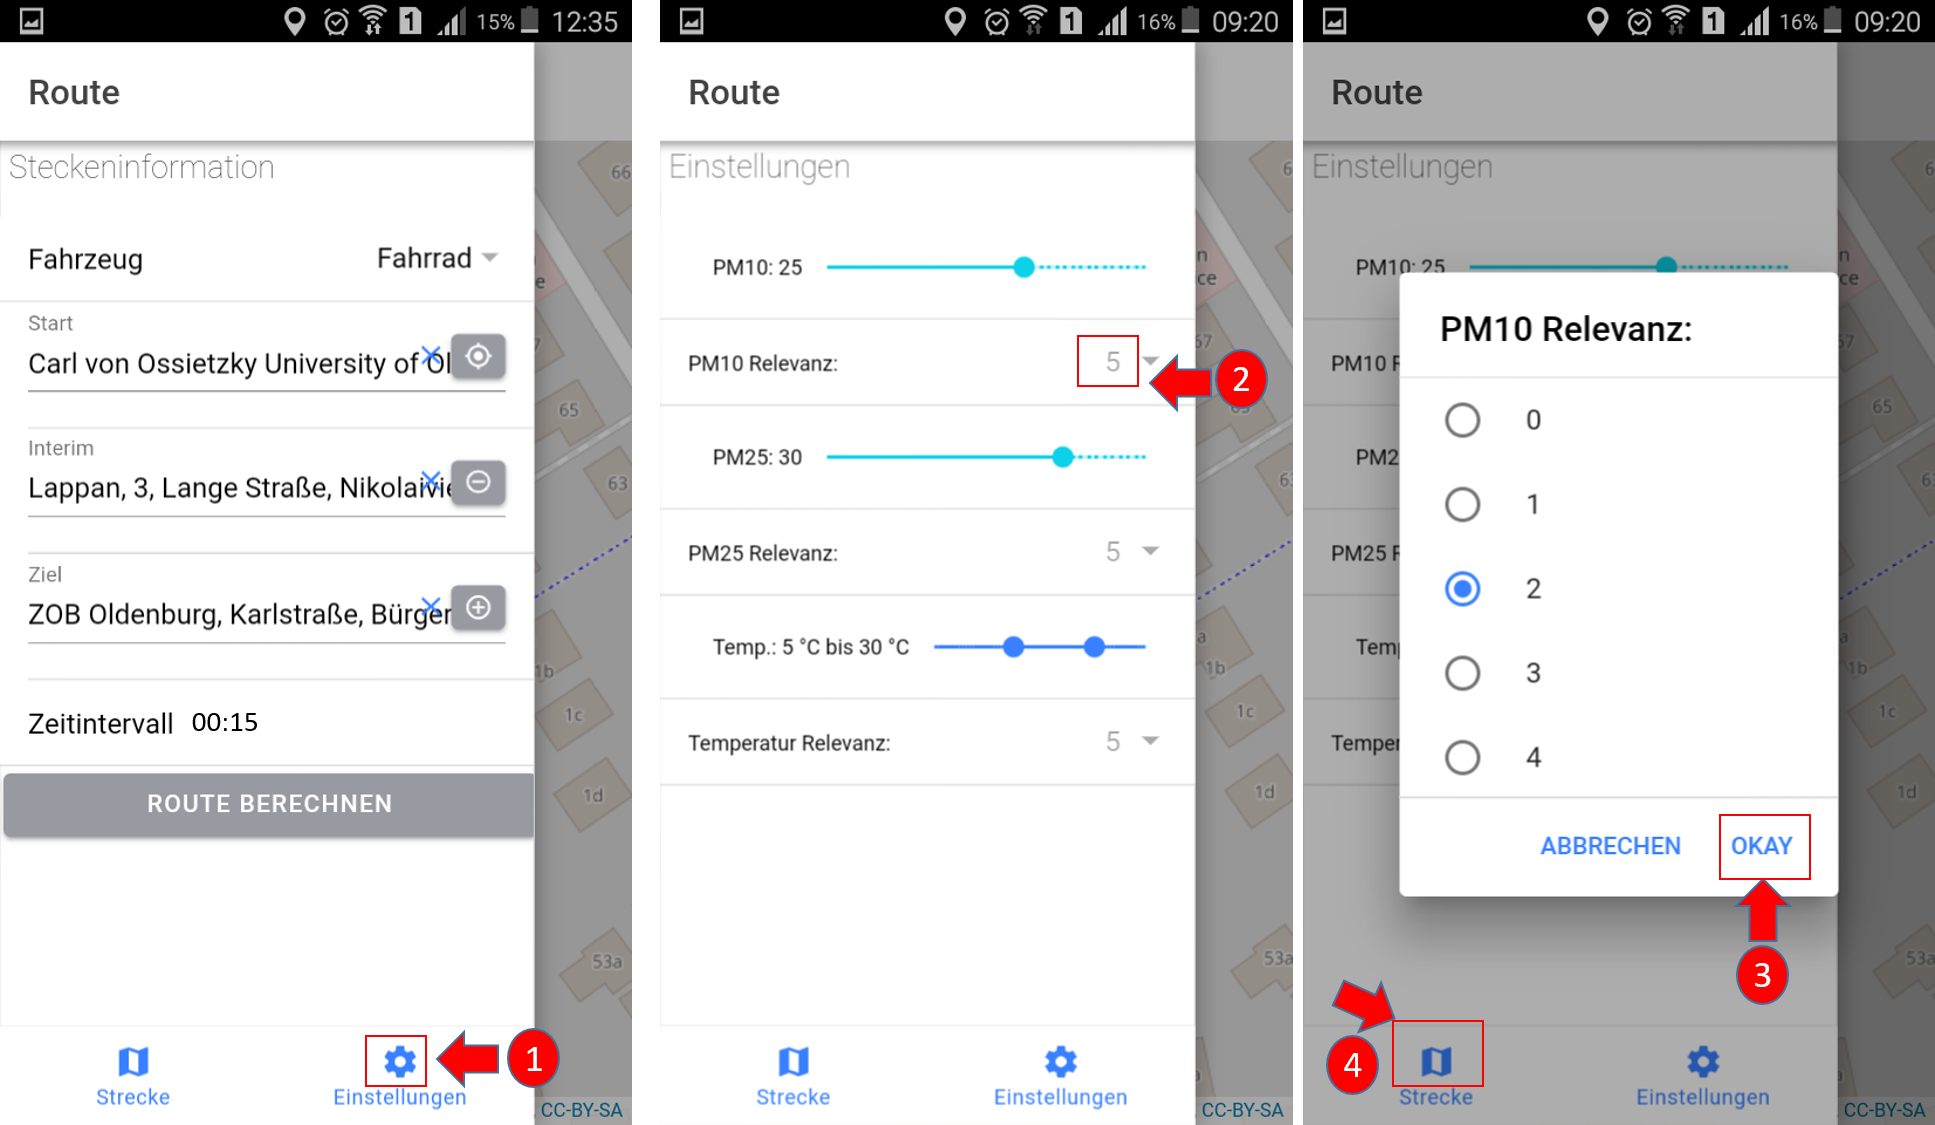
\includegraphics[height=8 cm]{./ressourcen/nutzerhandbuch/einstellungen.png}}
\caption{Routeneinstellungen}
\label{fig:app:Routeneinstellungen}
\end{figure} 

\newpage
\paragraph{Dynamisches Routing-Zeitintervall:}
In diesem Zeitintervall wird überprüft, ob es während der Navigation eine neue bessere Route gibt.\\
Wie gezeigt in \Fig{app:Dynamisches_Routing_Zeitintervall}.
\begin{figure}[h!]
\centerline{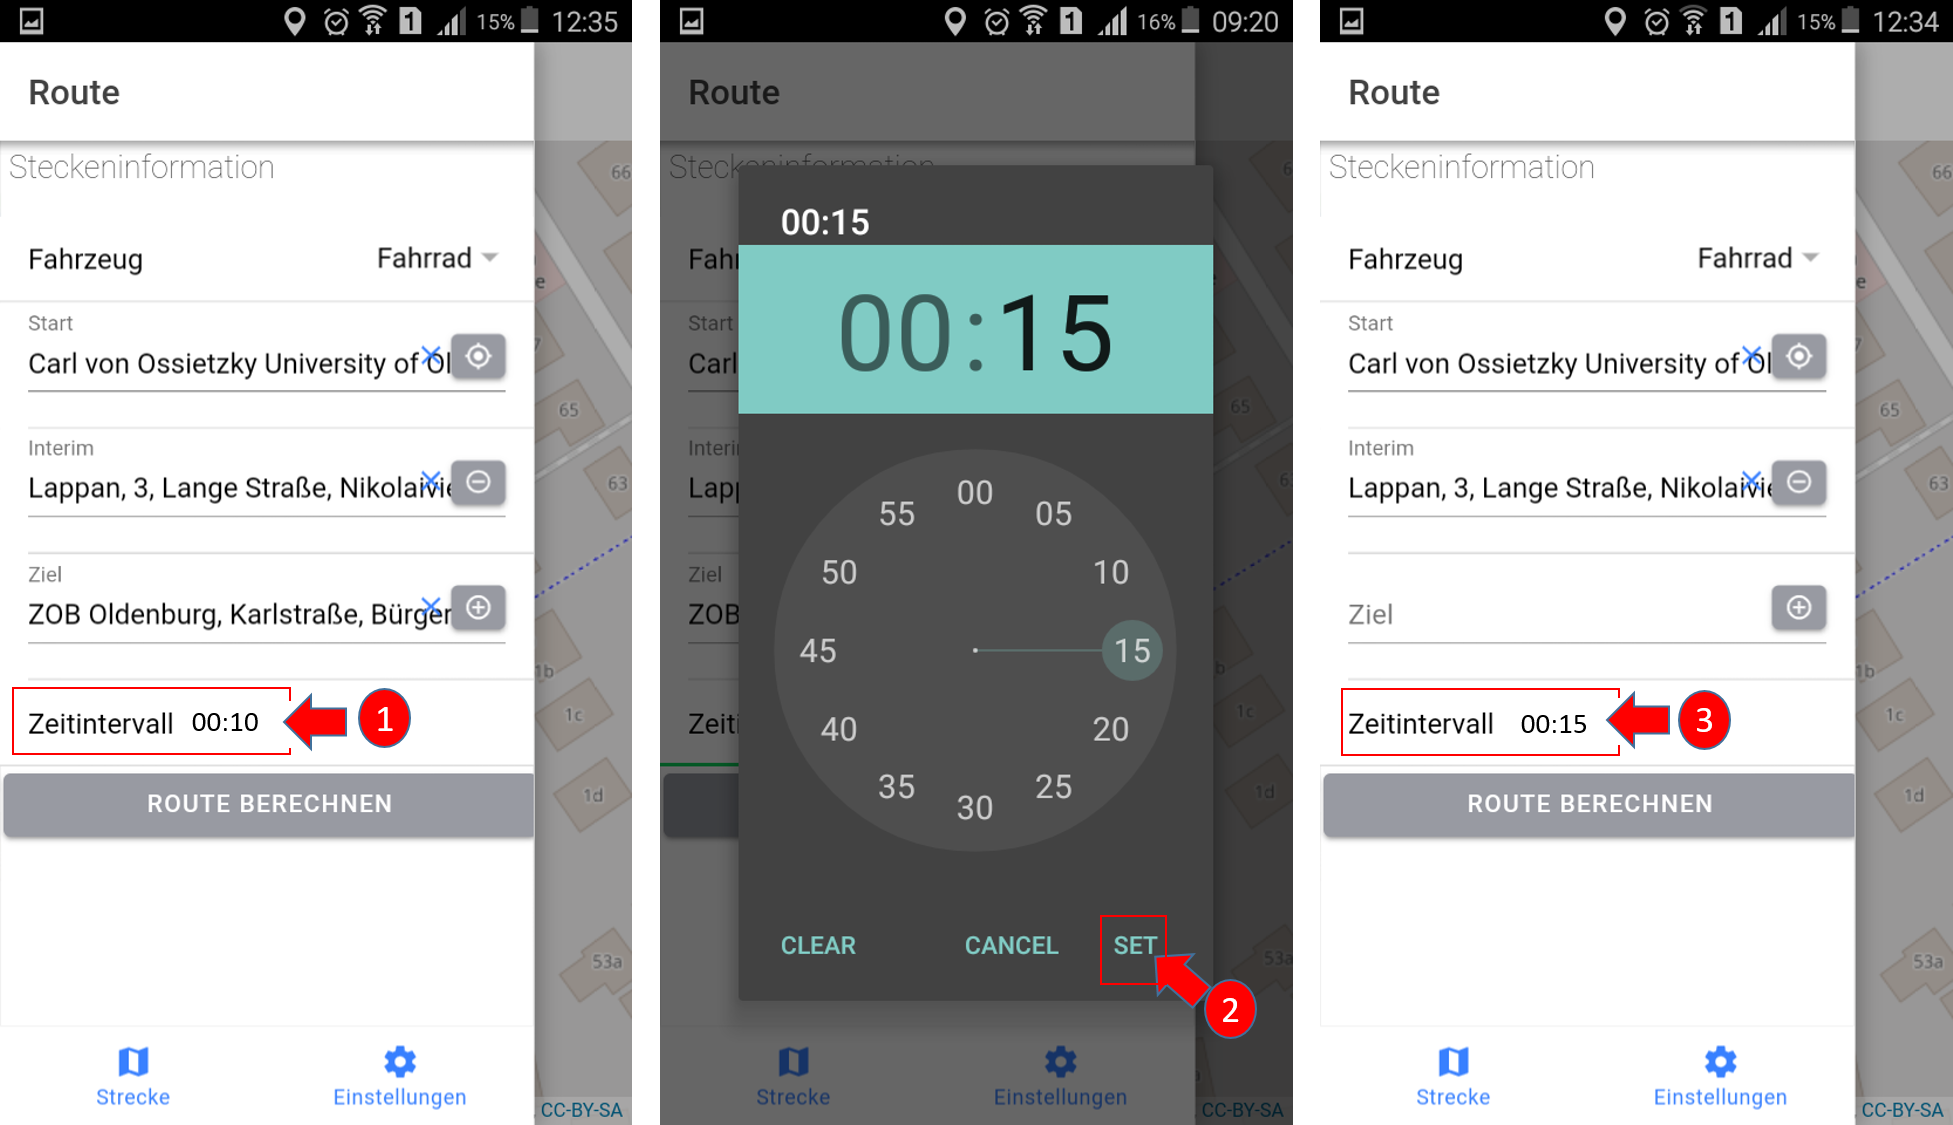
\includegraphics[height=6 cm]{./ressourcen/nutzerhandbuch/zeitintervall.png}}
\caption{Dynamisches Routing-Zeitintervall}
\label{fig:app:Dynamisches_Routing_Zeitintervall}
\end{figure} 

\paragraph{Fahrzeug:}
Wählen Sie Ihr Fahrzeug wie gezeigt in \Fig{app:Fahrzeug}.
\begin{figure}[h!]
\centerline{\includegraphics[height=6 cm]{./ressourcen/nutzerhandbuch/Fahrzeug.png}}
\caption{Fahrzeug}
\label{fig:app:Fahrzeug}
\end{figure} 


\paragraph{Route berechnen und Routen anzeigen:}
Nachdem Sie die Navigationspunkte ausgewählt haben, tippen Sie auf Route Berechnen, um eine Route zu berechnen.\\
Wie gezeigt in \Fig{app:route_berechnen_zwischen}.
\begin{itemize}
  \item Wenn die Navigationspunkte Zwischenziele enthalten, befindet sich nur eine Route zwischen dem Start und dem Ziel.
  
\begin{figure}[h!]
\centerline{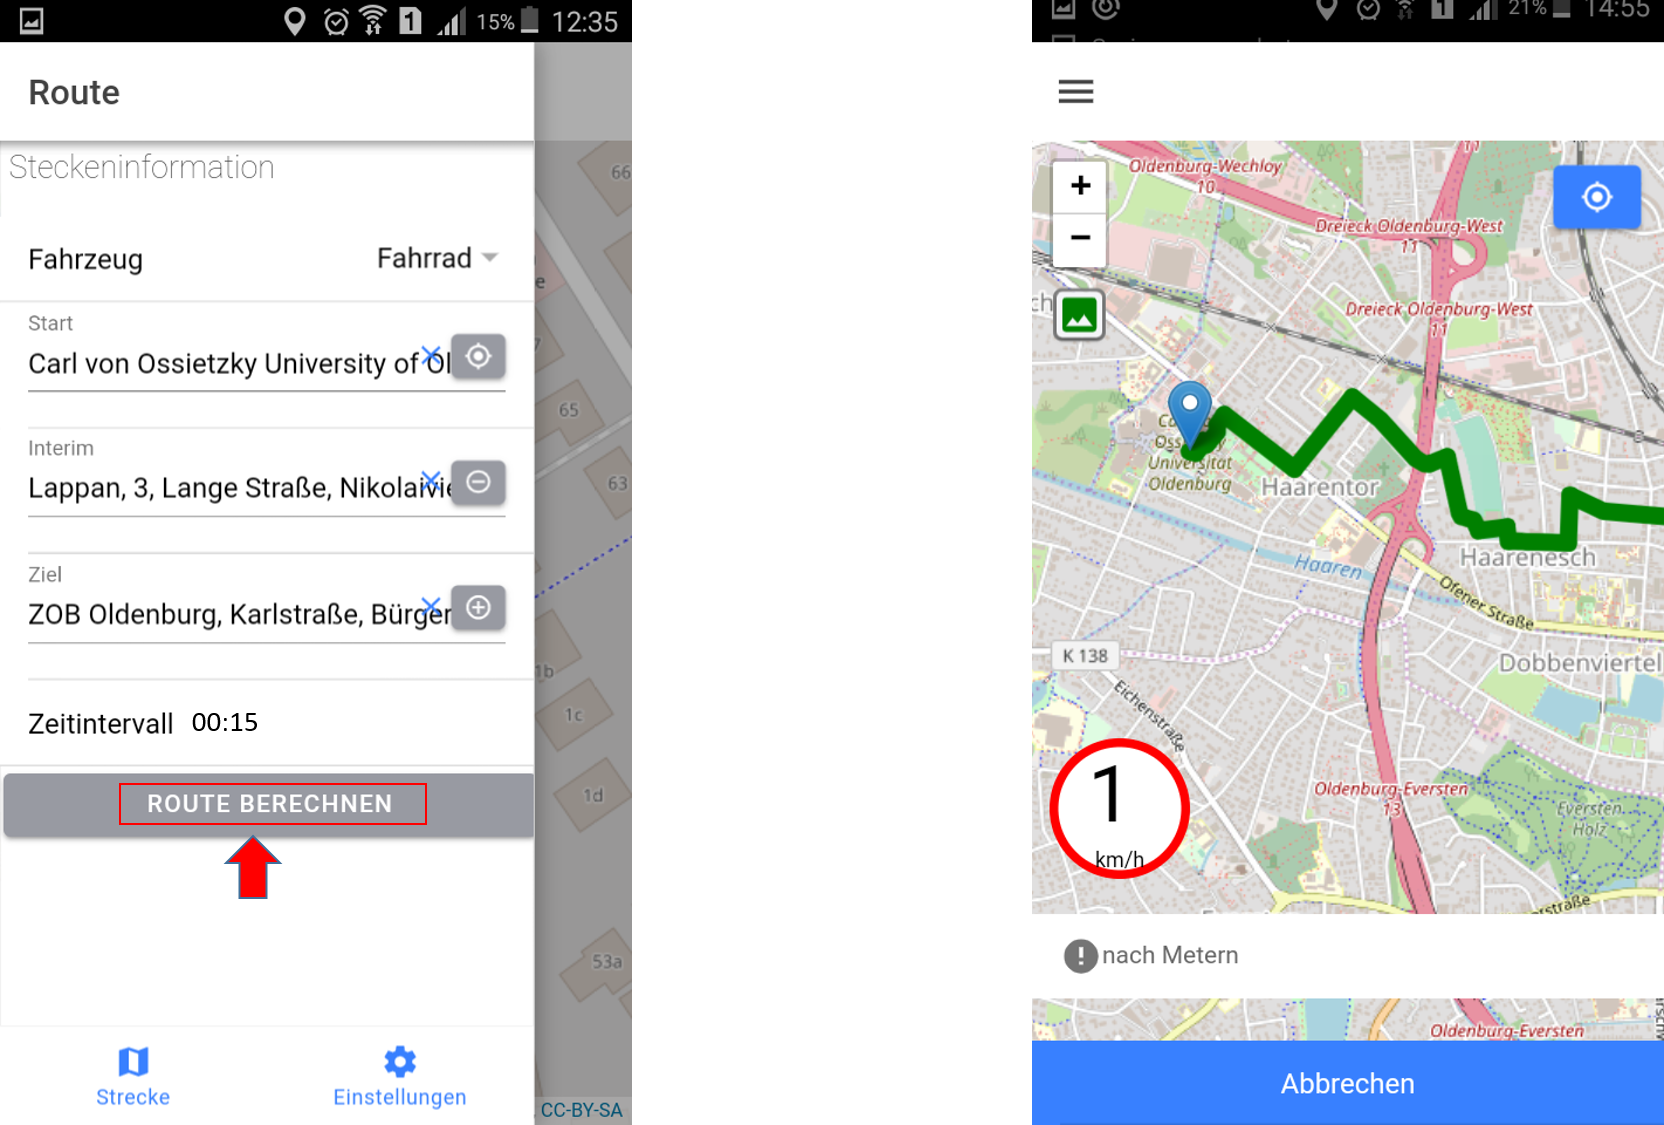
\includegraphics[height=8 cm]{./ressourcen/nutzerhandbuch/route_berechnen_zwischen.png}}
\caption{Route berechnen mit Zwischenziele}
\label{fig:app:route_berechnen_zwischen}
\end{figure} 

  \item Wenn die Navigationspunkte nur Start- und Zielpunkt enthälten, gibt es höchstens drei mögliche Routen.\\
  Wie gezeigt in \Fig{app:route_berechnen}.
  	\begin{itemize}
  		\item Um einen Route auszuwählen, tippen Sie auf die gewünschte Route.

  		\item Die beste Route ist grün, die zweitbeste blau und die drittbeste rot. Die gewählte Route ist visuell hervorgehoben.
	\end{itemize}
	
\begin{figure}[h!]
\centerline{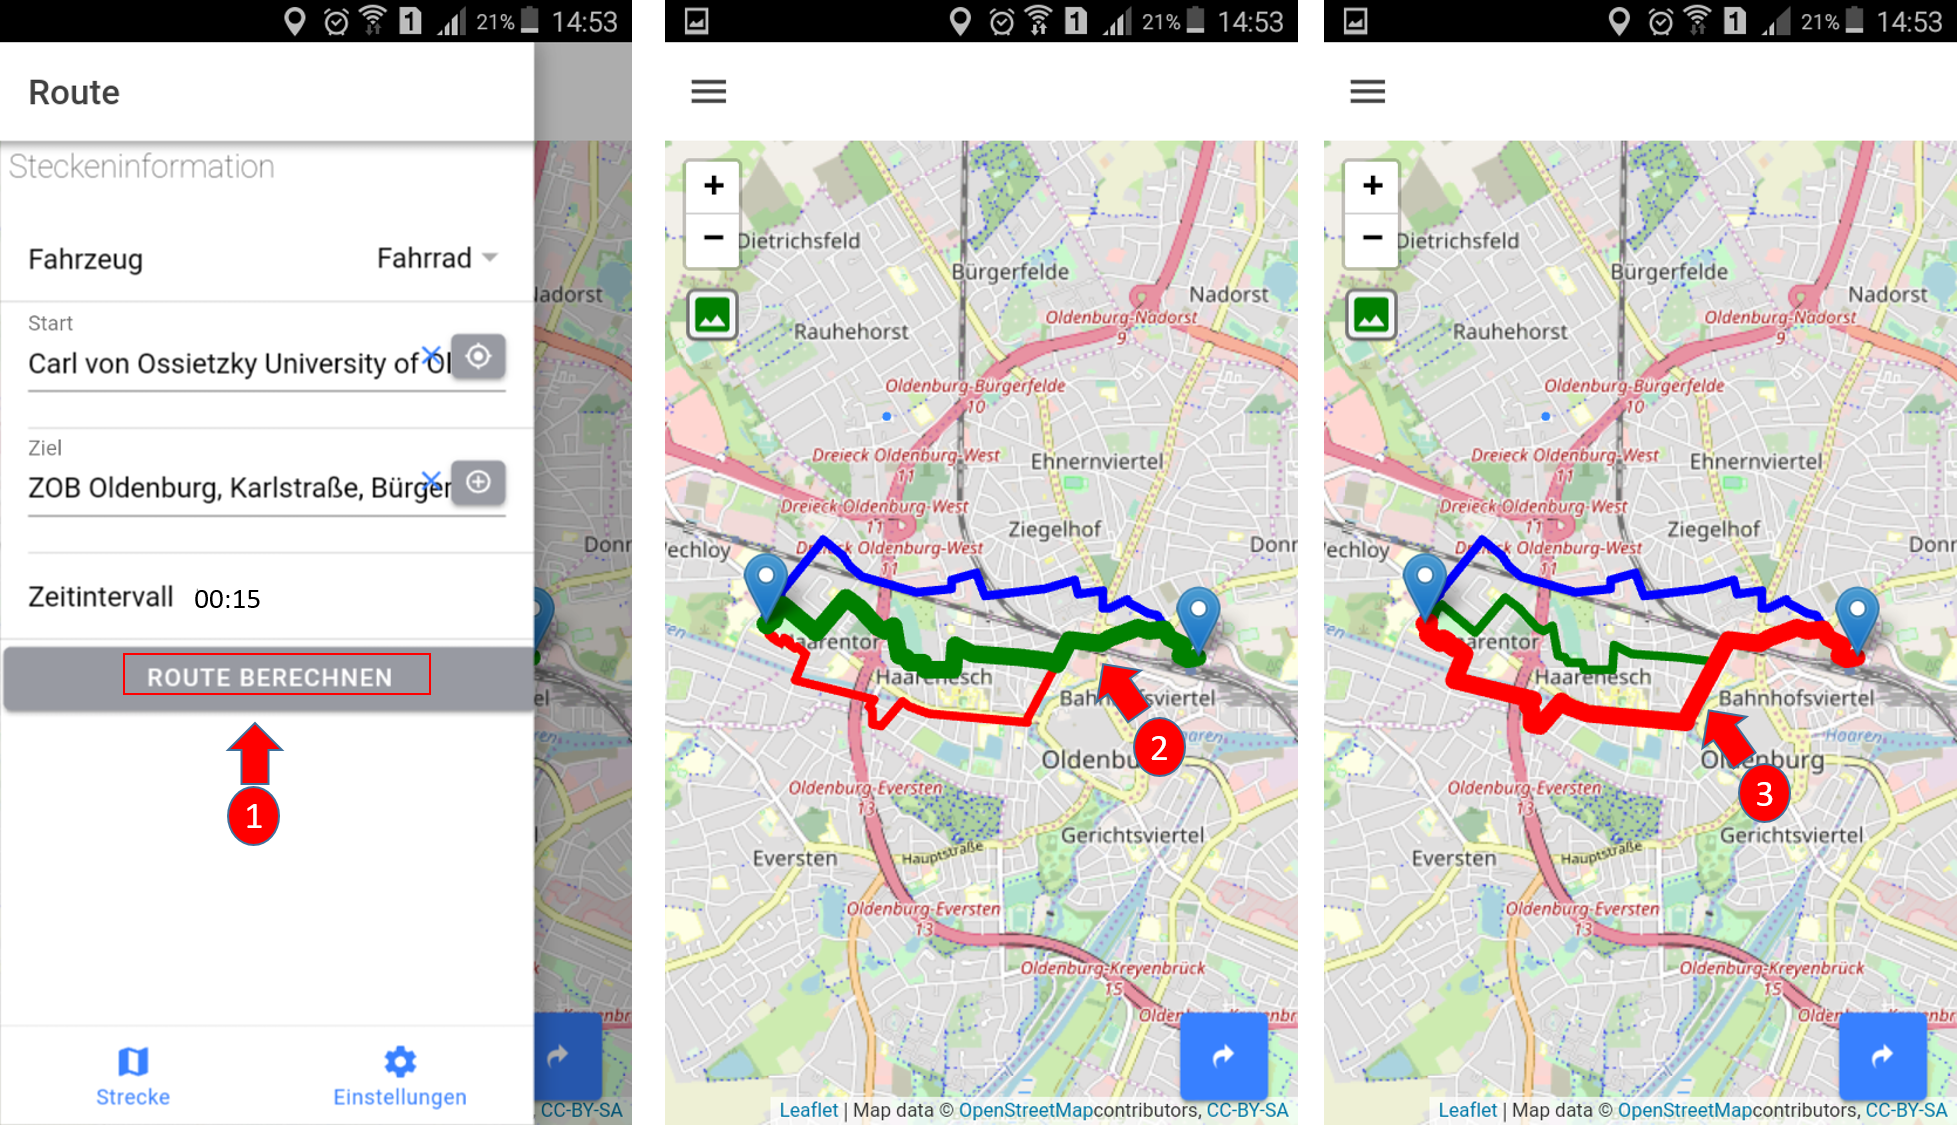
\includegraphics[height=8 cm]{./ressourcen/nutzerhandbuch/route_berechnen.png}}
\caption{Route berechnen ohne Zwischenziele}
\label{fig:app:route_berechnen}
\end{figure} 

\end{itemize}


\newpage
\paragraph{Navigieren:}
siehe \Fig{app:Navigieren}.
\begin{enumerate}
  \item Um die Navigation zu starten, tippen Sie auf die Navigationstaste. 
  \item Während der Navigation wird die aktuelle Position als blauer Kreis um die aktuelle Position angezeigt.
  \item Die Bewegungsgeschwindigkeit wird in einem roten Kreis links unten angezeigt.
  \item Die Navigationsanweisung wird unten angezeigt.
  \item Um die Navigation zu beenden, klicken Sie auf die Abbrechentaste.
  \item Wenn Sie auf die Navigationsanweisung klicken, wird eine Liste aller Navigationsanweisungen angezeigt.
\end{enumerate}

\begin{figure}[h!]
\centerline{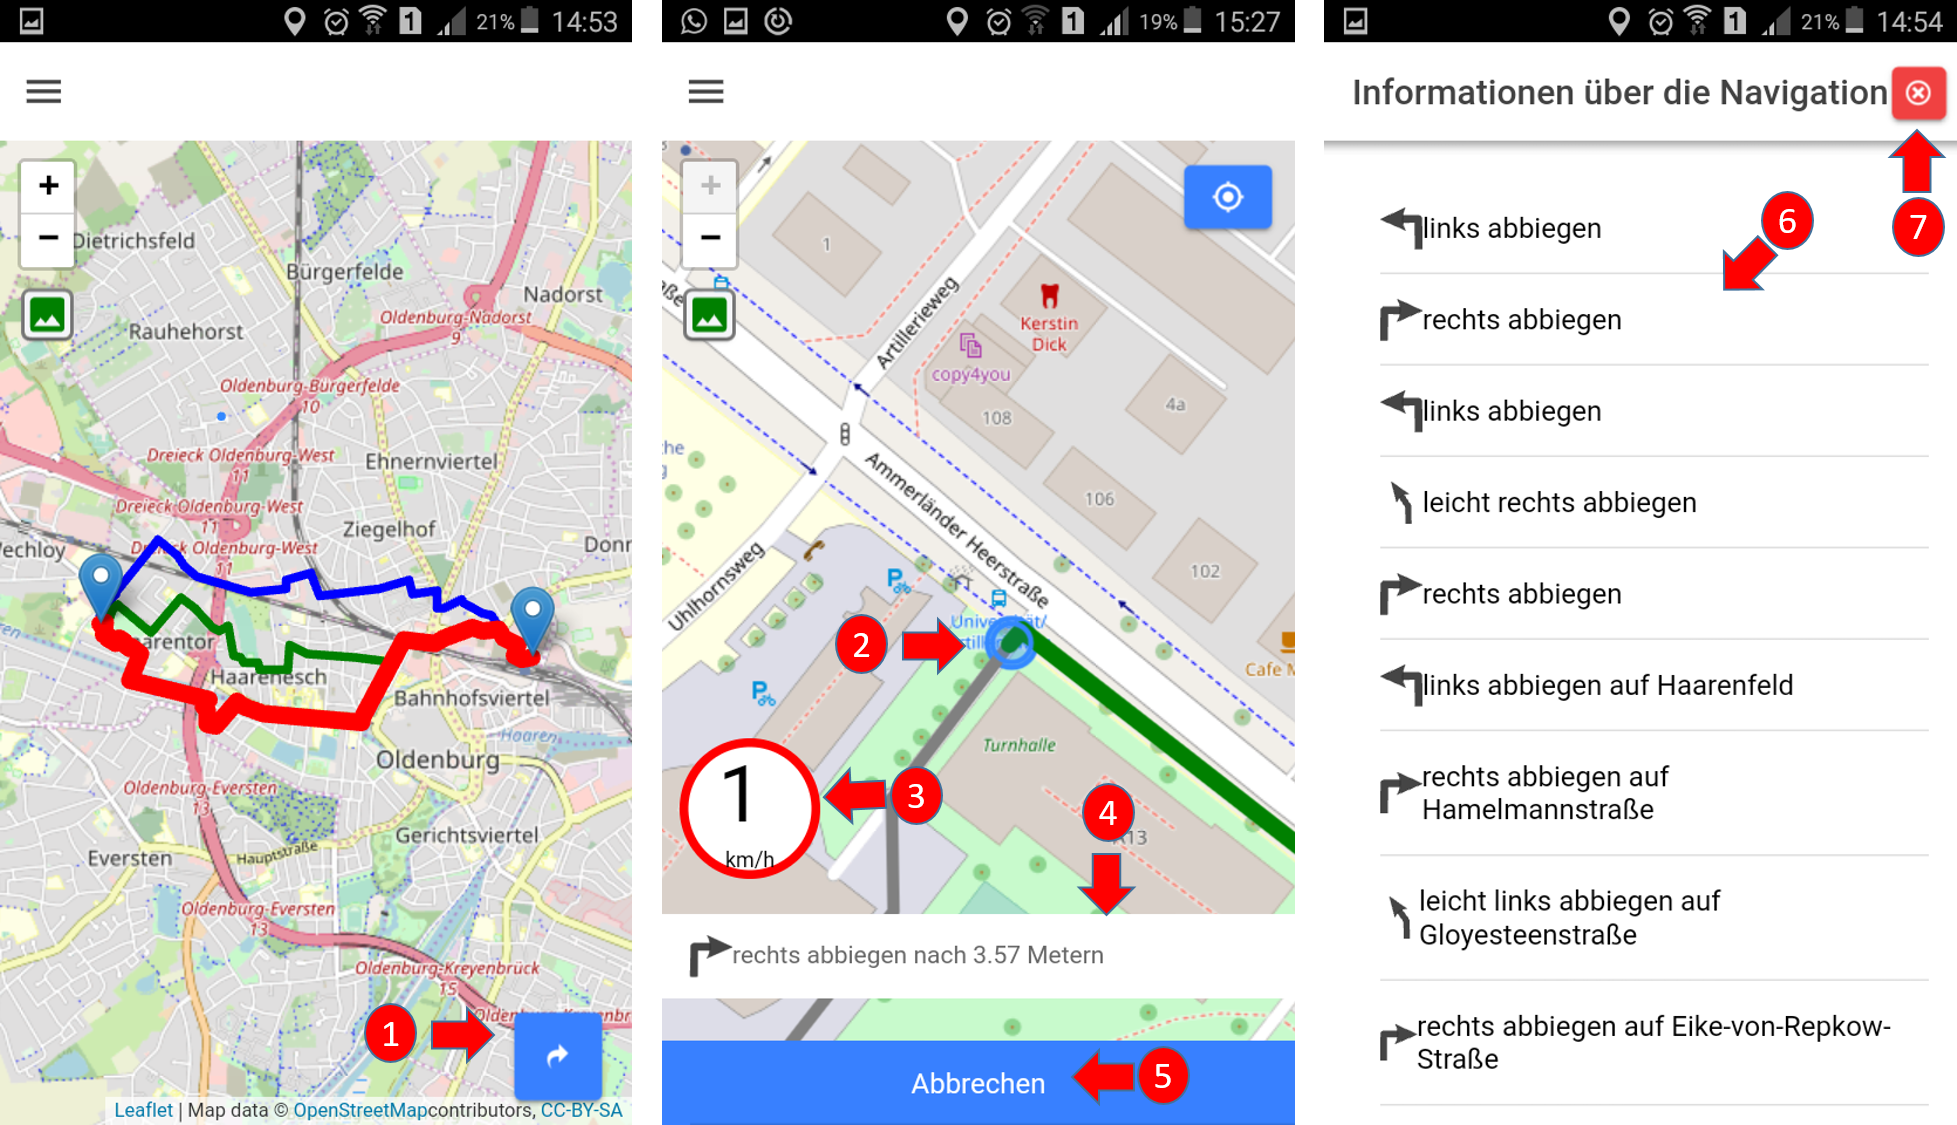
\includegraphics[height=8 cm]{./ressourcen/nutzerhandbuch/navigate.png}}
\caption{Navigieren}
\label{fig:app:Navigieren}
\end{figure}

\newpage
\paragraph{Heatmap:}
Um die Heatmap anzuzeigen, klicken Sie auf die Heatmap-Icon. Wie gezeigt in \Fig{app:heatmap}.\\
Die Heatmap zeigt, wie sich die Umgebungsparameter auf die Routenberechnung auswirken
\begin{figure}[h!]
\centerline{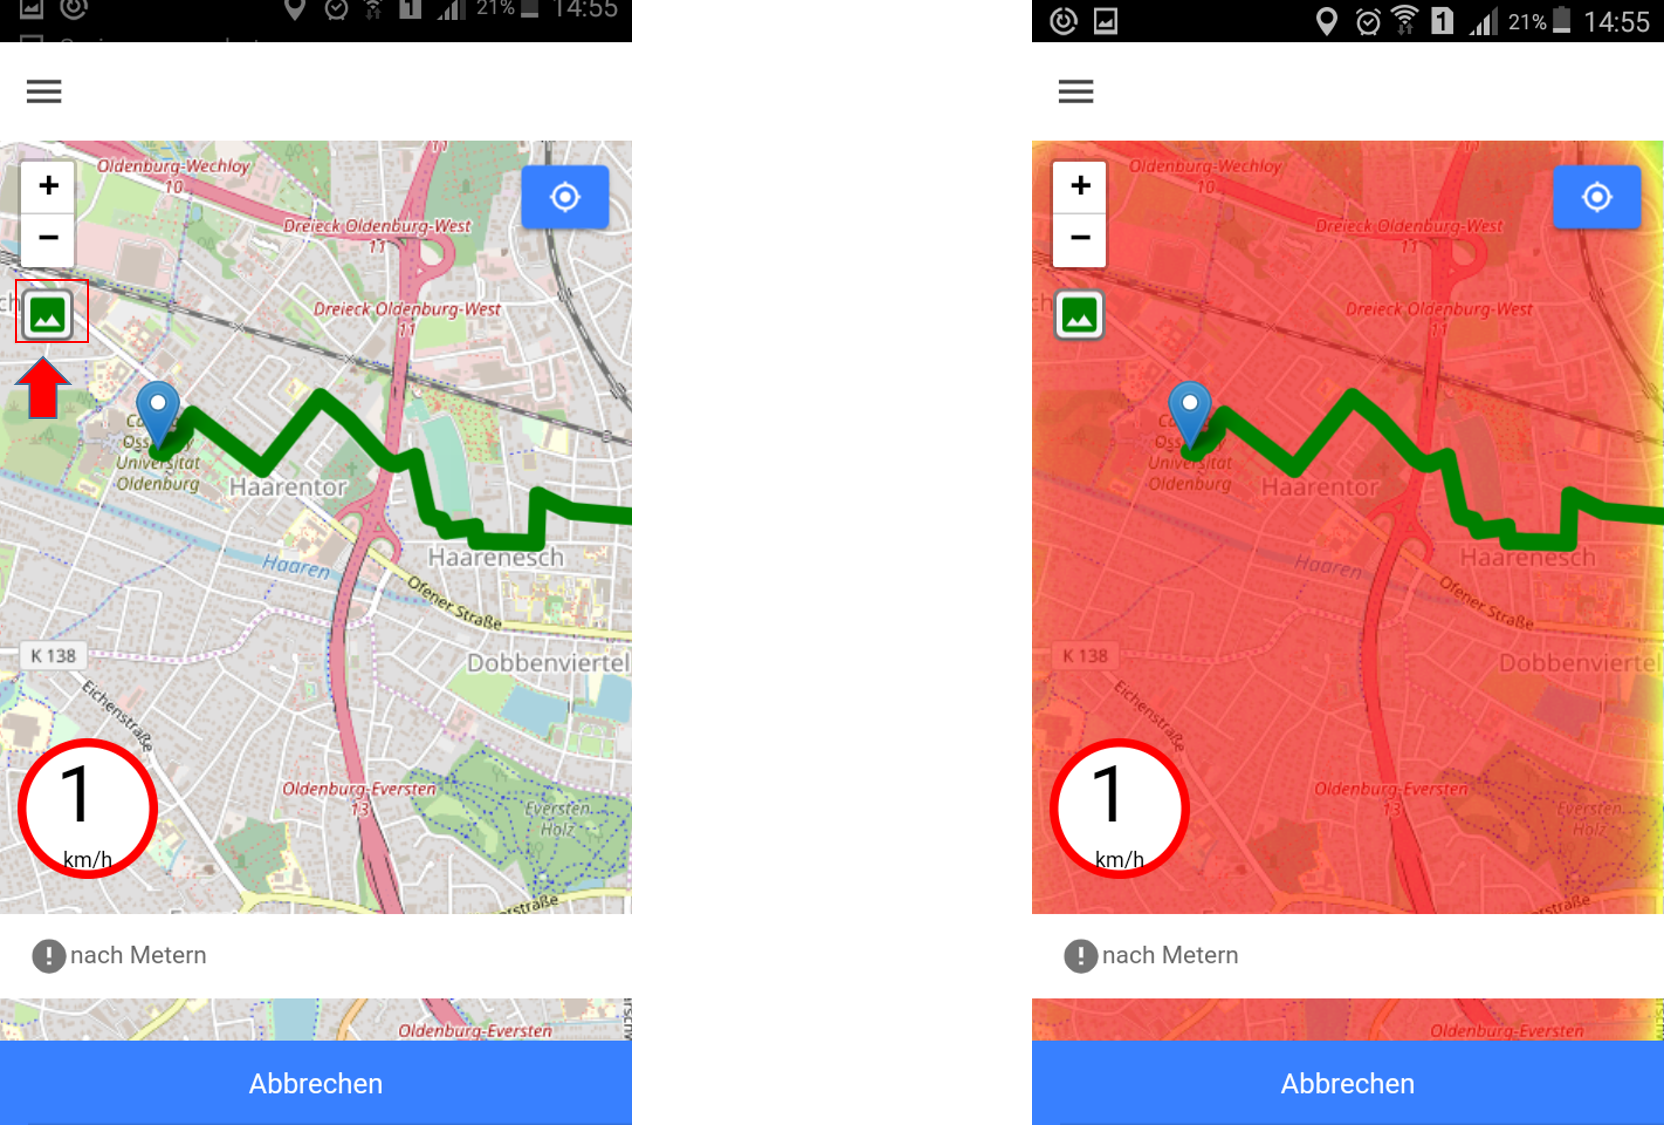
\includegraphics[height=6 cm]{./ressourcen/nutzerhandbuch/heatmap.png}}
\caption{heatmap}
\label{fig:app:heatmap}
\end{figure}
